\documentclass{article}
\usepackage{graphicx}
\usepackage{subcaption}
\usepackage{geometry}
\usepackage{tikz}
\usepackage{amsmath}
\usepackage{cleveref}
\usepackage{float}
\usepackage[useregional]{datetime2}
\def\checkmark{\tikz\fill[scale=0.4](0,.35) -- (.25,0) -- (1,.7) -- (.25,.15) -- cycle;}
\usepackage[font=small,skip=0pt]{caption}
\geometry{legalpaper, margin=1in}
\title{STAT 8003 Homework 2}
\author{Zhijia Chen}
\date{\today}

\begin{document}

\begin{titlepage}
    \maketitle
\end{titlepage}

\textbf{problem 1.}

\vspace{\baselineskip}
\textit{question 1.1.}

$$L(\alpha)=\prod_{i=1}^np(X_i|\alpha)=\prod_{i=1}^n\alpha\theta^\alpha X_i^{-\alpha-1}$$

\vspace{\baselineskip}
\textit{question 1.2.}

\begin{align*}
    l(\alpha)&=log(L(\alpha))\\
             &=\sum_{i=1}^n \left(log(\alpha)+\alpha log(\theta)-(\alpha+1)log(X_i)\right)\\
    l'(\alpha)&=\sum_{i=1}^n \left(\frac{1}{\alpha}+log(\theta)-log(X_i)\right)
\end{align*}

Solve $l'(\alpha)=0$, and we get $$\alpha=\frac{1}{\sum_{i=1}^n\left(\frac{log(X_i)}{n}-log(\theta)\right)}$$.

\vspace{\baselineskip}
\textit{question 1.3.}

\begin{align*}
    L(\theta)&=\prod_{i=1}^np(X_i|\theta)=\prod_{i=1}^n\alpha\theta^\alpha X_i^{-\alpha-1}\\
    l(\theta)&=\sum_{i=1}^n \left(log(\alpha)+\alpha log(\theta)-(\alpha+1)log(X_i)\right)\\
    l'(\theta)&=\frac{n\alpha}{\theta}
\end{align*}

Solve $l'(\theta)=0$...stuck here :(

\vspace{\baselineskip}
\textit{question 1.4.}

\begin{align*}
    E(x)&=\int_{x=\theta}^\infty x\alpha \theta^\alpha x^{-\alpha-1}dx\\
    &=\frac{\alpha\theta^\alpha}{1-\alpha}\int_{x=\theta}^\infty (1-\alpha)x^{-\alpha}dx\\
    &=\frac{\alpha\theta^\alpha}{1-\alpha}\bigg|_{\theta}^{\infty}\\
    &=\lim_{x\to\infty}\frac{\alpha\theta^\alpha}{1-\alpha}\left(x^{1-\alpha}-\theta^{1-\alpha}\right) 
\end{align*}

Since we assume $\alpha>1$, $E(x)=\frac{\alpha\theta}{\alpha-1}=\frac{3\alpha}{\alpha-1}$.

\begin{align*}
    \overline{X_i}&=\frac{3\alpha}{\alpha-1}\\
    \alpha&=\frac{\overline{X_i}}{\overline{X_i}-3}
\end{align*}

\vspace{\baselineskip}
\textit{question 1.5.}

See figure 1.

\begin{figure}[H]
    \centering
        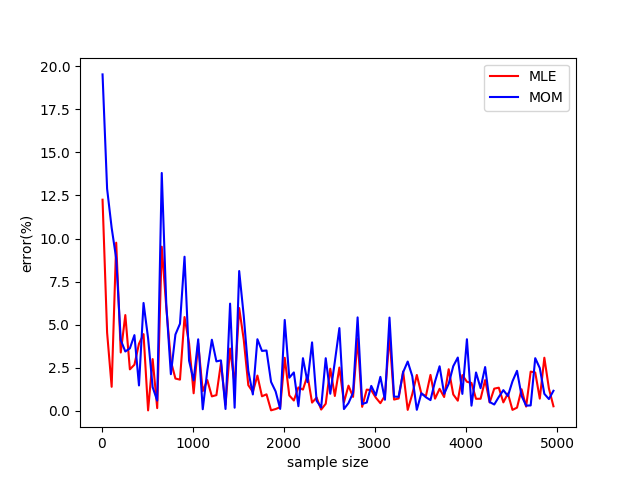
\includegraphics[width=0.5\textwidth]{2-1-5}
    \caption{question 1.5.}
    \label{fig:1-5}
\end{figure}

\end{document}

